%\documentclass{beamer}
\documentclass[10pt,english,t,10pt]{beamer}
\beamertemplatenavigationsymbolsempty

\usepackage{amsfonts}
\usepackage{amsmath}
\usepackage{bbm}
%\usepackage{graphicx}
%\usepackage{listings}
\usepackage{epstopdf}
\usepackage{booktabs}
\usepackage{bigstrut}
\usepackage{rotating}
\usepackage{multirow}
\usepackage{threeparttable}
\usepackage{caption} % subcaption
\usepackage{hyperref}
%\usepackage{tikz}


\usepackage[utf8]{inputenc}
\usepackage[T1]{fontenc}
\usepackage{amsmath}
\usepackage{amsfonts}
\usepackage{amssymb}
\usepackage{mhchem}
\usepackage{stmaryrd}
\usepackage{graphicx}
\usepackage[export]{adjustbox}


\newenvironment{wideitemize}{\itemize\addtolength{\itemsep}{10pt}}{\enditemize}
\newenvironment{wideenumerate}{\enumerate\addtolength{\itemsep}{10pt}}{\endenumerate}


%% LyX 2.3.6.1 created this file.  For more info, see http://www.lyx.org/.
%% Do not edit unless you really know what you are doing.

\usepackage{lmodern}
\usepackage[T1]{fontenc}
\usepackage[utf8]{inputenc}
\setcounter{tocdepth}{1}
\setlength{\parskip}{\smallskipamount}
\setlength{\parindent}{0pt}
\usepackage{units}
\usepackage{amstext}
\usepackage{amssymb}
\usepackage{graphicx}
\usepackage[authoryear]{natbib}
\PassOptionsToPackage{normalem}{ulem}
\usepackage{ulem}

\makeatletter
%%%%%%%%%%%%%%%%%%%%%%%%%%%%%% Textclass specific LaTeX commands.
% this default might be overridden by plain title style
\newcommand\makebeamertitle{\frame{\maketitle}}%
% (ERT) argument for the TOC
\AtBeginDocument{%
	\let\origtableofcontents=\tableofcontents
	\def\tableofcontents{\@ifnextchar[{\origtableofcontents}{\gobbletableofcontents}}
	\def\gobbletableofcontents#1{\origtableofcontents}
}

%%%%%%%%%%%%%%%%%%%%%%%%%%%%%% User specified LaTeX commands.



\usepackage{tikz}
\usetikzlibrary{positioning}
\usepackage{appendixnumberbeamer}

\usepackage{graphicx}
\usepackage{subfig}

\usetheme[progressbar=frametitle,block=fill,subsectionpage=progressbar]{metropolis}

% margin
\setbeamersize{text margin right=1.5cm}

% colors
\colorlet{DarkRed}{red!70!black}
\setbeamercolor{normal text}{fg=black}
\setbeamercolor{alerted text}{fg=DarkRed}
\setbeamercolor{progress bar}{fg=DarkRed}
\setbeamercolor{button}{bg=DarkRed}

% width of seperators
\makeatletter
\setlength{\metropolis@titleseparator@linewidth}{1pt}
\setlength{\metropolis@progressonsectionpage@linewidth}{1pt}
\setlength{\metropolis@progressinheadfoot@linewidth}{1pt}
\makeatother

% new alert block
\newlength\origleftmargini
\setlength\origleftmargini\leftmargini
\setbeamertemplate{itemize/enumerate body begin}{\setlength{\leftmargini}{4mm}}
\let\oldalertblock\alertblock
\let\oldendalertblock\endalertblock
\def\alertblock{\begingroup \setbeamertemplate{itemize/enumerate body begin}{\setlength{\leftmargini}{\origleftmargini}} \oldalertblock}
\def\endalertblock{\oldendalertblock \endgroup}
\setbeamertemplate{mini frame}{}
\setbeamertemplate{mini frame in current section}{}
\setbeamertemplate{mini frame in current subsection}{}
\setbeamercolor{section in head/foot}{fg=normal text.bg, bg=structure.fg}
\setbeamercolor{subsection in head/foot}{fg=normal text.bg, bg=structure.fg}

% footer
\makeatletter
\setbeamertemplate{footline}{%
	\begin{beamercolorbox}[colsep=1.5pt]{upper separation line head}
	\end{beamercolorbox}
	\begin{beamercolorbox}{section in head/foot}
		\vskip1pt\insertsectionnavigationhorizontal{\paperwidth}{}{\hskip0pt plus1filll \insertframenumber{} / \inserttotalframenumber \hskip2pt}\vskip3pt% 
	\end{beamercolorbox}%
	\begin{beamercolorbox}[colsep=1.5pt]{lower separation line head}
	\end{beamercolorbox}
}
\makeatother

% toc
\setbeamertemplate{section in toc}{\hspace*{1em}\inserttocsectionnumber.~\inserttocsection\par}
\setbeamertemplate{subsection in toc}{\hspace*{2em}\inserttocsectionnumber.\inserttocsubsectionnumber.~\inserttocsubsection\par}


% Automatically create vspace between items
% See: https://tex.stackexchange.com/questions/369504/beamer-vertically-stretching-level-1-list-items-in-a-nested-list-environment
%\usepackage{xpatch} 
%\xpatchcmd{\itemize}   
%	{\def\makelabel}   
%	{\ifnum\@itemdepth=1\relax      
%		\setlength\itemsep{\fill} % separation for first level    
%		\fi\def\makelabel   
%	}{}{} 
%\xpatchcmd{\enditemize}   
%	{\endlist}   
%	{\endlist\ifnum\@itemdepth<2\else\vfil\fi}{}{}




%% Automatically create vspace between items
%% See: https://jayrobwilliams.com/posts/2019/10/better-beamer
%\makeatletter
%\renewcommand{\itemize}[1][]{%
%	\beamer@ifempty{#1}{}{\def\beamer@defaultospec{#1}}%
%	\ifnum \@itemdepth >2\relax\@toodeep\else
%	\advance\@itemdepth\@ne
%	\beamer@computepref\@itemdepth% sets \beameritemnestingprefix
%	\usebeamerfont{itemize/enumerate \beameritemnestingprefix body}%
%	\usebeamercolor[fg]{itemize/enumerate \beameritemnestingprefix body}%
%	\usebeamertemplate{itemize/enumerate \beameritemnestingprefix body begin}%
%	\list
%	{\usebeamertemplate{itemize \beameritemnestingprefix item}}
%	{\def\makelabel##1{%
%			{%
%				\hss\llap{{%
%						\usebeamerfont*{itemize \beameritemnestingprefix item}%
%						\usebeamercolor[fg]{itemize \beameritemnestingprefix item}##1}}%
%			}%
%		}%
%	}
%	\fi%
%	\setlength\itemsep{\fill}
%	\ifnum \@itemdepth >1
%	\vfill
%	\fi%  
%	\beamer@cramped%
%	\raggedright%
%	\beamer@firstlineitemizeunskip%
%}
%
%\def\enditemize{\ifhmode\unskip\fi\endlist%
%	\usebeamertemplate{itemize/enumerate \beameritemnestingprefix body end}
%	\ifnum \@itemdepth >1
%	\vfil
%	\fi%  
%}
%\makeatother
%
%\makeatother

\usepackage{babel}
\begin{document}
	\title{7. Wealth Inequality \vspace{-2mm}}
	\subtitle{Adv. Macro: Heterogenous Agent Models} 
	\author{Jeppe Druedahl \& Patrick Moran}
	\date{2023}
	
	{
		\setbeamertemplate{footline}{} 
		\begin{frame}
		
		\maketitle
		
		\begin{tikzpicture}[overlay, remember picture]
		\node[above left=0cm and 0.0cm of current page.south east] 
		{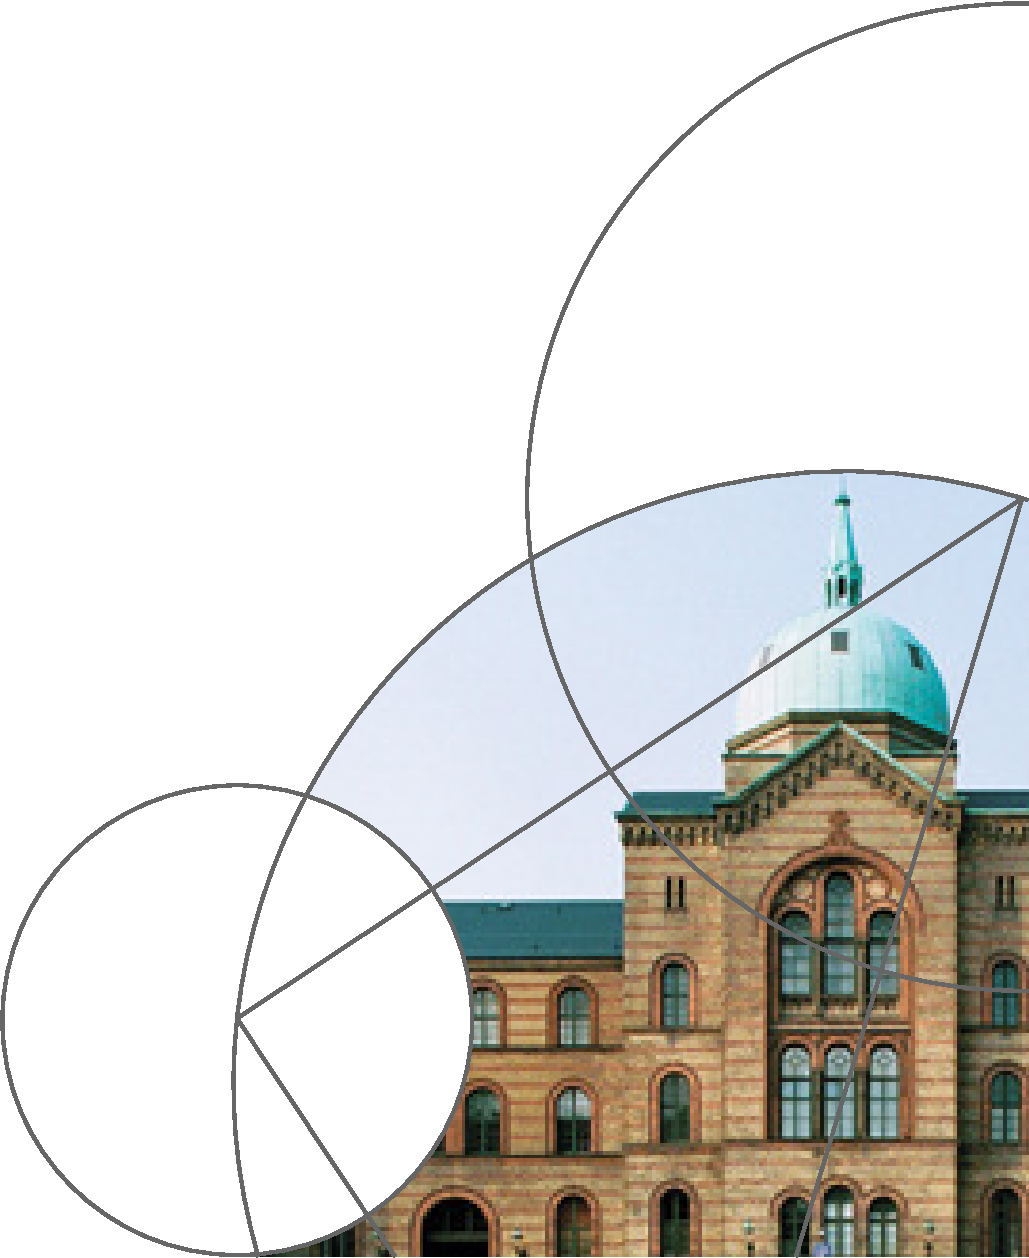
\includegraphics[width=4cm]{figs/KUSAMFtitlelrcorner.pdf}};
		\end{tikzpicture}
		
		\begin{tikzpicture}[overlay, remember picture]
		\node[below left=0.5cm and .8cm of current page.north east] 
		{\includegraphics[width=1.5cm]{figs/KUSAMFlogo.pdf}};
		\end{tikzpicture}
		
		\begin{tikzpicture}[overlay, remember picture]
		\node[below right=0.5cm and 0.8cm of current page.north west] 
		{
\includegraphics[width=1.5cm]{figs/CEBI.png}};
		\end{tikzpicture}
		
		\begin{tikzpicture}[overlay, remember picture]
		\node[above right=0.5cm and 0.8cm of current page.south west] 
		{
\includegraphics[width=1.5cm]{figs/DNRF.png}};
		\end{tikzpicture}
		
	\end{frame}
}

\addtocounter{framenumber}{-1}


\section{Introduction}

\begin{frame}{Wealth Inequality}
\vspace{-2mm}
\begin{itemize}
\item <+->\textbf{Goal for today:} Better understand wealth inequality 
through the lens of heterogeneous agent general equilibrium models \vfill
\item <+->\textbf{Central economic questions:}
\begin{enumerate}
	\item Why are some people rich while others are poor?
	\item To what extent can governments affect inequality?
%	What does the baseline Aiyigari model predict in terms of wealth inequality?
%	\item How can we augment the baseline model to obtain a closer match of reality?
	\item What explains the rise in wealth inequality in recent decades? \vfill
\end{enumerate}

\item <+->To answer these questions, we need to better understand why people save, and how this translates into wealth inequality \vfill

\item <+->\textbf{Plan for today:}
\begin{enumerate}
	\item Study the predictions of a baseline Bewley-Huggett-Aiyagari model
	\item Consider various model extensions that help match the data
	\item Then use such a model to better understand the rise in wealth inequality in the US 
\end{enumerate}
\end{itemize}
\end{frame}
%

\begin{frame}{Note}
\vspace{-2mm}

\vspace{20mm}
\begin{itemize}
	\item The views expressed in this presentation are those of the author
	and do not represent the views of the Federal Reserve Board or Federal
	Reserve System.
\end{itemize}
\end{frame}

%\begin{document}
%\frame{\titlepage}


\section{Savings and Wealth Inequality}


%\begin{frame}
%\frametitle{Important open questions}
%
%
%
%Which instruments should they use?
%
%To better answer these questions we need to better understand why people save
%
%
%\end{frame}




%\begin{frame}
%\frametitle{First half of lecture today}
%
%Why do people save?
%
%How does saving behavior translate into wealth inequality?
%
%\end{frame}


%\begin{frame}
%\frametitle{Roadmap}
%
%Basic facts
%
%Basic Bewley-Huggett-Aiyagari-Imrohoroglu model
%
%Richer models
%
%What have have learned so far about savings?
%
%
%
%\end{frame}


\subsection{Basic Facts}
\begin{frame}
\frametitle{Earnings and wealth inequality}
\begin{itemize}
	\item Skewed distributions with thick upper tails
	
	\item Wealth more concentrated than earnings
	
\end{itemize}

\pause
\begin{center}
\begin{tabular}{lccccc}
	\hline\hline
	& \quad\quad & \quad\quad & \quad\quad &  \quad\quad &  Percent at zero \\
	& Top $1 \%$ & Top $5 \%$ & Top $20 \%$ & Top $40 \%$ & or negative \\
	\hline
	Wealth & 29 & 53 & 80 & 93 & 6 \\
	
	Earnings & 6 & 19 & 48 & 72 & 8 \\
	\hline\hline
\end{tabular}
\end{center}

\pause
\begin{itemize}
	\item Wealth and earnings becoming more concentrated over time
	
	\item Rich people (high lifetime income, education, wealth) have a higher saving rate before and after retirement
	
\end{itemize}
\end{frame}



\begin{frame}
\frametitle{Wealth more concentrated than earnings}


Not only in the US, but also Denmark and almost all other countries

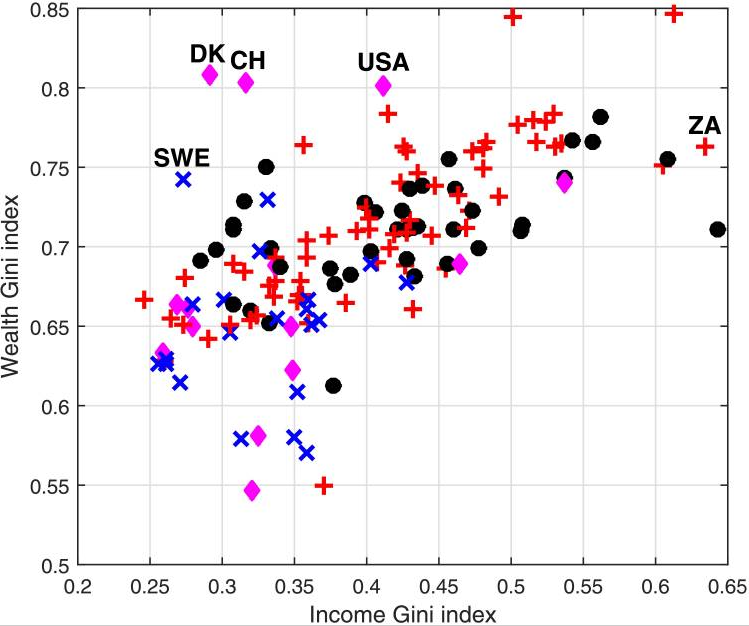
\includegraphics[width=0.75\textwidth]{figs/Cross-Country-Gini.png}
% Figure from https://www.ncbi.nlm.nih.gov/pmc/articles/PMC4841595/

\end{frame}



\begin{frame}
\frametitle{Quick refresher: Gini index}


\begin{itemize}
	\item Measures extent a distribution deviates from perfect equality
	
	\item 0 represents perfect equality, 1 implies perfect inequality
	
	\item Gini Index = $\frac{A}{A+B}$
	
\end{itemize}

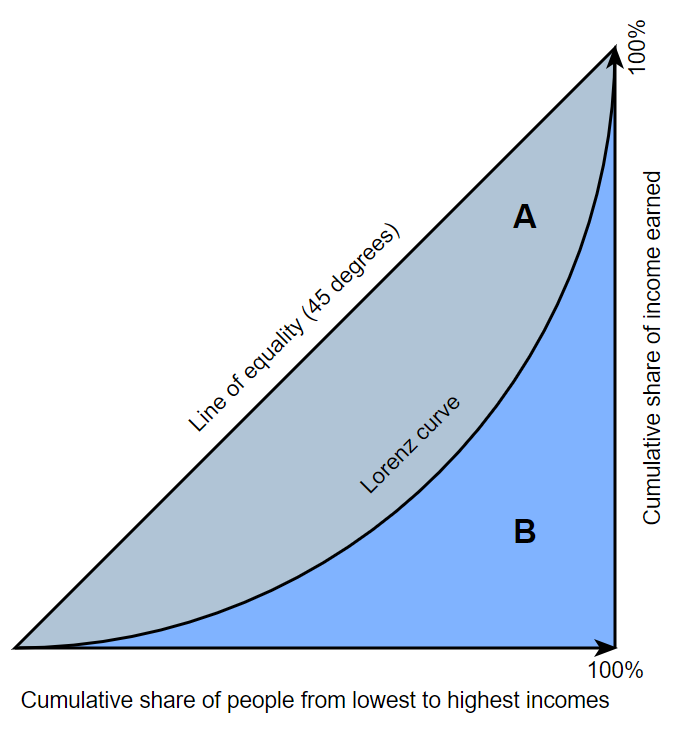
\includegraphics[width=0.5\textwidth]{figs/Gini.png}

\begin{itemize}
	\item Wealth and earnings becoming more concentrated over time
	
	\item Rich people (high lifetime income, education, wealth) have a higher saving rate before and after retirement
	
\end{itemize}
\end{frame}




\subsection{Basic models of inequality}

\begin{frame}
\frametitle{Aiyagari Model}

\begin{itemize}
	\item Infinitely lived agents
	
	\item Preferences
\end{itemize}
$$
\max _{\left\{c_{t}\right\}_{t=0}^{\infty}} E \sum_{t=0}^{\infty} \beta^{t} \frac{c_{t}^{1-\sigma}}{1-\sigma}
$$

\begin{itemize}
\item Budget constraint
\end{itemize}
$$
a_{t+1}=y_{t}+(1+r) a_{t}-c_{t}, \quad a_{t+1} \geq \underline{a}
$$

\begin{itemize}
\item Ex-ante identical households hit by earning shocks

\item Households are ex-post heterogeneous

\item Constant distribution of people over states (assets, age) and individuals face a lot of uncertainty

\end{itemize}

\end{frame}



\begin{frame}
\frametitle{Aiyagari Model}


\begin{tabular}{lcccc}
	\hline 
	& \text { Wealth Gini } & \multicolumn{3}{l}{\text { Wealth in top (\%) }} \\
	& \cline { 2 - 4 } & & 1 \% & 5 \% & 20 \% \\
	\hline 
	\text { U.S. data, } 1989 \text { SCF } & & & & \\
	& .78 & 29 & 53 & 80 \\
	\text { Aiyagari Baseline } &  & & & \\
	& .38 & 3.2 & 12.2 & 41.0 \\
	\text { Aiyagari higher variability } & &  & & \\
	& .41 & 4.0 & 15.6 & 44.6 \\
	\hline
\end{tabular}

\end{frame}


%--------------------------------------
\begin{frame}
\frametitle{Finitely lived agents (Huggett model)}
\begin{itemize}
	\item Finitely lived agents with overlapping generations
\item Preferences
\end{itemize}
$$
\max _{\left\{c_{t}\right\}_{t=0}^{T}} E \sum_{t=0}^{T} s_{t} \beta^{t} \frac{c_{t}^{1-\sigma}}{1-\sigma}
$$

\begin{itemize}
	\item $s_t$ is the survival probability 	
	
	\item Budget constraint
\end{itemize}
$$
a_{t+1}=y_{t}+(1+r) a_{t}-c_{t}, \quad a_{t+1} \geq \underline{a}
$$


\begin{itemize}

	\item $y_{t}$ is an exogenous, age-dependent earnings process 

	\begin{itemize}
		\item Stochastic hump shaped income profile over the working life, then flat income stream after exogenous retirement
	\end{itemize}
%\item Households are ex-post heterogeneous
%
%\item Constant distribution of people over states (assets, age) and individuals face a lot of uncertainty

%\item Aggregate production function $F(K, L) = A K^\alpha L^{1−\alpha}$


\end{itemize}
\end{frame}

%--------------------------------------
\begin{frame}
\frametitle{Closing the model}
\begin{itemize}
	\item Aggregate production function $ Y_{t}=A K_{t-1}^{\alpha}L_{t}^{1-\alpha}$ (w/ exog. $L=1$)
	
%	$	F(K, L)=AK^\alpha L^{1−\alpha}$
	
	
	\item A stationary equilibrium is given by
	

\begin{enumerate}	
	\item  Quantities $K_{ss}$ % and $L_{ss}$, 
	\item  interest rate $r_{ss}$ % and $w_{ss}$,	
	\item  the distribution $\boldsymbol{D}_{ss}$ over $y_{t}$ and $a_{t-1}$
	\item  and the policy functions $a_{ss}^{\ast}(z_{t},a_{t-1})$ and $c_{ss}^{\ast}(z_{t},a_{t-1})$	
\end{enumerate}

\pause
	are such that
	
\begin{enumerate}	
	\item Household maximize expected utility (policy functions)
	\item Firms maximize profits (prices)
	\item $\boldsymbol{D}_{ss}$ is the invariant distribution implied by the HH problem
%	\item The labor market clears
	\item The capital market clears
	\item The goods market clears
\end{enumerate}	
	
	
%	
%	\item an interest rate r and wage rate w,
%	\item  allocations c(x), a'(x),
%	\item government tax rates and transfers (τa, τl, τb, exb, p),
%	\item and a constant distribution of people over the state variables x: m*(x)
	
\end{itemize}
\end{frame}

%--------------------------------------
\begin{frame}
\frametitle{Results}

\begin{itemize}
	\item The Huggett model succeeds in matching the US Gini coefficient
\end{itemize}

\begin{tabular}{lc|ccccc|c}
	\hline 
	& \text { Wealth } & \multicolumn{5}{c}{\text { Wealth in top (\%) }} & Share with \\
	& Gini  & 1 \% & 5 \% & 20 \% & 40\% & 60\% & wealth $\leq 0$ \\
	\hline 
	\text { US data} & & & & && & \\
	& .78 & 29 & 53 & 80 & 93 & 98 & 6 \\
	\text { Model } &  & & & && & \\
	& .67 & 7 & 27 & 69 & 90 & 98 & 17\\
	\hline
\end{tabular}

\pause 
\vfill 
\begin{itemize}
	
	\item But this is achieved by having: 
	\begin{itemize}
		\item too many people holding little wealth
		\item not by concentrating wealth in the right tail of the wealth distribution
	\end{itemize}
\end{itemize}

\end{frame}




%--------------------------------------
\begin{frame}
\frametitle{Key mechanism}
\begin{wideitemize}
\item Precautionary savings behavior. People save to self-insure against

\begin{itemize}
\item Earnings risk

\item Longevity risk

\item Retirement
\end{itemize}


\item Once "buffer stock savings" is reached, people start dissaving. Carroll (1997)

\item In the model: The saving rate of the high wealth households is low or even negative

\begin{itemize}
\item Contrasts with much empirical evidence (Dynan Skinner and Zeldes, 2004 and De Nardi, French and Jones, 2010)
\end{itemize}


\end{wideitemize}
\end{frame}

%--------------------------------------
\begin{frame}
\frametitle{Model-implied saving rate by age and wealth}
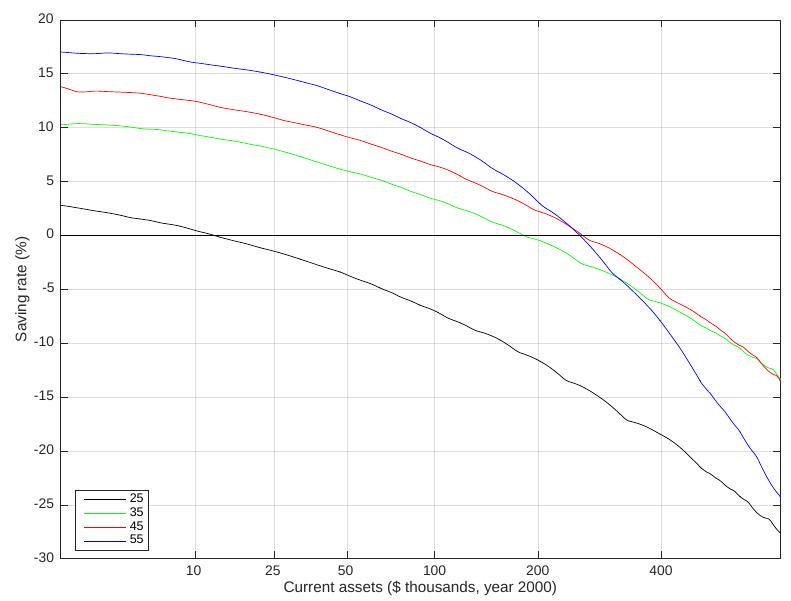
\includegraphics[max width=\textwidth]{DeNardiFella-Figs/2022_10_05_feede24bac33b2bb1aaag-04}

Standard life cycle Bewley model

\end{frame}


%--------------------------------------
\begin{frame}
\frametitle{Limitations of the standard model}
\begin{wideitemize}
\item Model generates counterfactual saving behavior

\item Model does not generate enough high wealth people as in the data

\item Model allows for very few saving motives. Might miss important saving motives 

\item Why people save is important

\end{wideitemize}
\end{frame}



\section{Richer Models of Inequality}


%--------------------------------------
\begin{frame}
\frametitle{Explaining wealth inequality}
$$
\begin{gathered}
\max _{\left\{c_{t}\right\}_{t=0}^{T}} E \sum_{t=0}^{T} \beta^{t}\left(s_{t} \frac{c_{t}^{1-\sigma}}{1-\sigma}+ \textcolor{blue}{\left(1-s_{t}\right) s_{t-1} \phi\left(a_{t}\right)} \right) \\
a_{t+1}= \textcolor{blue}{y_{t}} +(1+r) a_{t}-c_{t}+\textcolor{blue}{b_{t}}, \quad a_{t+1} \geq \underline{a}
\end{gathered}
$$

\begin{enumerate}
\item Bequests and human capital transmission across generations
\end{enumerate}
\end{frame}



%--------------------------------------
\begin{frame}
\frametitle{Explaining wealth inequality}
$$
\begin{gathered}
\max _{\left\{c_{t}\right\}_{t=0}^{T}} E \sum_{t=0}^{T} \textcolor{blue}{\beta_{i}}^{t} s_{t} \frac{c_{t}^{1-\textcolor{blue}{\sigma_{i}}}}{1-\textcolor{blue}{\sigma_{i}}} \\
a_{t+1}=y_{t}+(1+r) a_{t}-c_{t}, \quad a_{t+1} \geq \underline{a}
\end{gathered}
$$

\begin{enumerate}
\item 
\item Heterogeneous preferences

\end{enumerate}
\end{frame}


%--------------------------------------
\begin{frame}
\frametitle{Explaining wealth inequality}
$$
\begin{gathered}
\max _{\left\{c_{t}\right\}_{t=0}^{T}} E \sum_{t=0}^{T} \beta^{t} s_{t} \frac{c_{t}^{1-\sigma}}{1-\sigma} \\
a_{t+1}=\textcolor{blue}{\left[l_{e} f\left(\theta_{t}, k_{t}\right)+\left(1-l_{e}\right) y_{t}\right]}+(1+r)\left(a_{t}-k_{t}\right)-c_{t}, \quad a_{t+1} \geq \underline{a}
\end{gathered}
$$

\begin{enumerate}
	\item 
	\item 
	\item Entrepreneurship
\end{enumerate}
\end{frame}

%--------------------------------------
\begin{frame}
\frametitle{Explaining wealth inequality}
$$
\begin{gathered}
\max _{\left\{c_{t}\right\}_{t=0}^{T}} E \sum_{t=0}^{T} \beta^{t} s_{t} \frac{c_{t}^{1-\sigma}}{1-\sigma} \\
a_{t+1}=y_{t}+\left(1+\textcolor{blue}{r_{t}^{i}}\right) a_{t}-c_{t}, \quad a_{t+1} \geq \underline{a}
\end{gathered}
$$

\begin{enumerate}
\item 
\item 
\item 
\item Idiosyncratic rates of return

\end{enumerate}
\end{frame}







%--------------------------------------
%\begin{frame}
%\frametitle{Explaining wealth inequality}
%$$
%\begin{gathered}
%\max _{\left\{c_{t}\right\}_{t=0}^{T}} E \sum_{t=0}^{T} \beta^{t} s_{t} \frac{c_{t}^{1-\sigma}}{1-\sigma} \\
%a_{t+1}=\textcolor{blue}{y_{t}}+(1+r)\left(a_{t}-k_{t}\right)-c_{t}, \quad a_{t+1} \geq \underline{a}
%\end{gathered}
%$$
%
%\begin{enumerate}
%\item 
%\item 
%\item 
%\item 
%\item Richer earnings dynamics
%
%\end{enumerate}
%\end{frame}




\subsection{Bequests}
%--------------------------------------
\begin{frame}
\frametitle{Bequests and human capital, facts}
\begin{itemize}
\item A large fraction of wealth is inherited
Kotlikoff and Summers (1981), Modigliani (1988), Gale and Scholz (1994)
\item Earnings of parents and children are correlated Solon (1992), Zimmermann (1992), Stokey (1996),... Chetty et al. (2014)
\end{itemize}
\end{frame}



%--------------------------------------
\begin{frame}
\frametitle{Bequests and human capital model (De Nardi, 2004)}
\begin{itemize}
\item OLG with retirement period.

\item Earnings and lifetime uncertainty. Accidental bequests

\item Parents value leaving bequests. Voluntary bequests
\pause 
\item Children partially inherit parents' earnings ability

pause 

\end{itemize}
$$
\begin{gathered}
\max _{\left\{c_{t}\right\}_{t=0}^{T}} E \sum_{t=0}^{T} \beta^{t}\left(s_{t} \frac{c_{t}^{1-\sigma}}{1-\sigma}+ \textcolor{blue}{\left(1-s_{t}\right) s_{t-1} \phi\left(a_{t}\right)} \right) \\
a_{t+1}= \textcolor{blue}{y_{t}} +(1+r) a_{t}-c_{t}+\textcolor{blue}{b_{t}}, \quad a_{t+1} \geq \underline{a}
\end{gathered}
$$

\end{frame}



%--------------------------------------
\begin{frame}
\frametitle{The bequest motive}
\begin{itemize}
\item "Warm glow altruism."
\end{itemize}
$$
\phi\left(a_{t}\right)=\frac{\left(a_{t}+\eta\right)^{1-\sigma}}{1-\sigma}
$$

\begin{itemize}
\item The larger is $\eta$, the more bequests are luxury goods. Non-homoteticity

\pause 

\begin{itemize}
\item Many people leave no bequests. Hurd and Smith (2001)

\item The altruistic model has strong implications about risk sharing across generations that have been strongly rejected by data, Altonji, Hayashi, Kotlikoff, 1997
\end{itemize}

\item Do not pick model parameters to match wealth inequality

\end{itemize}
\end{frame}



%%--------------------------------------
%\begin{frame}
%\frametitle{Data and basic Bewley life cycle model}
%\begin{tabular}{ccccccccc}
%\hline\hline
%Wealth & \multicolumn{7}{c}{Percentage wealth in the top} & $\% \leq 0$ \\
%Gini & $1 \%$ & $5 \%$ & $20 \%$ & $40 \%$ & $60 \%$ & Wealth &  &  \\
%\hline
%U.S. data, SCF & 1989 &  &  &  &  &  &  &  \\
%$.78$ & 29 & 53 & 80 & 93 & 98 & 6 &  &  \\
%\hline
%Accidental bequests distributed equally to all &  &  &  &  &  &  &  &  \\
%$.67$ & 7 & 27 & 69 & 90 & 98 & 17 &  &  \\
%\hline
%Accidental bequests distributed to one's children &  &  &  &  &  &  &  &  \\
%$.68$ & 7 & 27 & 69 & 91 & 99 & 17 &  &  \\
%\hline\hline
%\end{tabular}
%
%\end{frame}


%--------------------------------------
\begin{frame}
\frametitle{Age profiles of wealth by quantiles}
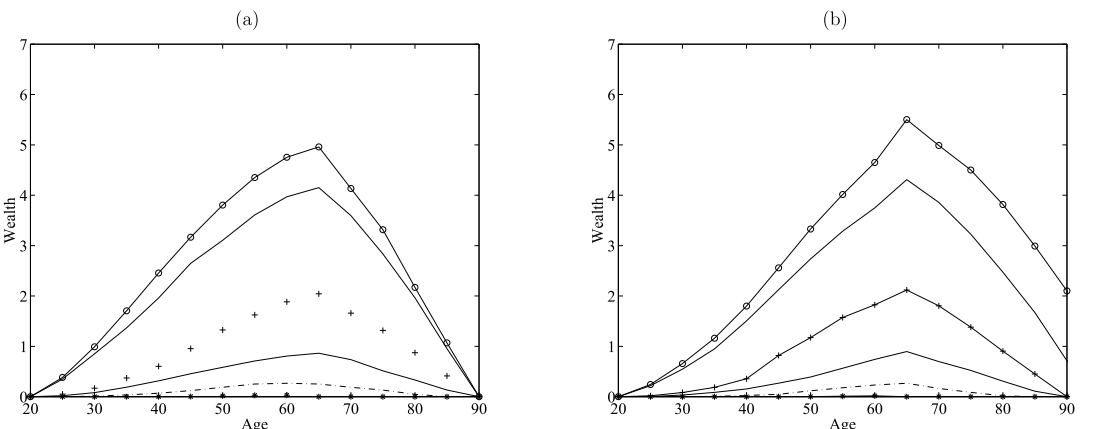
\includegraphics[max width=\textwidth]{DeNardiFella-Figs/Bequest-age-profiles.png}

\begin{itemize}
	\item A: No bequests - households spend all wealth in retirement
	\item B: Bequest motive - rich households maintain substantial wealth for children
\end{itemize}
\end{frame}

%--------------------------------------
\begin{frame}
\frametitle{Data and richer life cycle model}
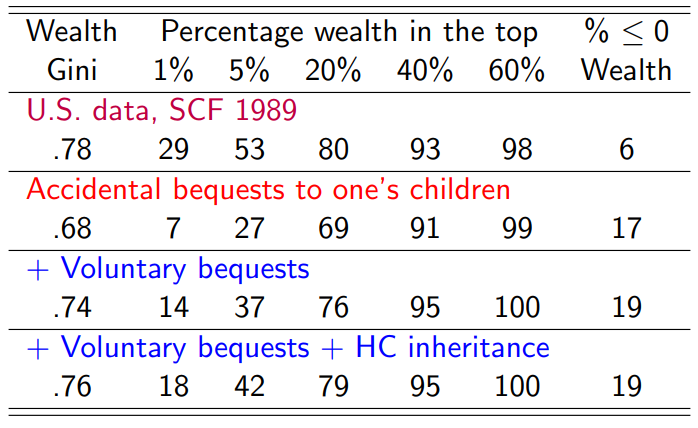
\includegraphics[max width=\textwidth]{DeNardiFella-Figs/Bequests.png}

\end{frame}



%--------------------------------------
\begin{frame}
\frametitle{Bequests and human capital: main results}
\begin{wideitemize}
\item Accidental bequests do not help explain the concentration in the upper tail of the wealth distribution

\item Voluntary bequests help explain wealth concentration because of non-homoteticity

\pause 
\item Transmission of earnings ability across generations increases wealth concentration in the upper tail

\pause 

\item But, the wealthy in the model are still not wealthy enough and the poor are too poor


\end{wideitemize}
\end{frame}


\subsection{Heterogeneous preferences}
%--------------------------------------
\begin{frame}
\frametitle{Heterogeneous preferences, facts}
Lots of evidence of preference heterogeneity

\begin{wideitemize}
\item Estimate Euler equations. PSID. Lawrence (1991).

\item Estimate life cycle model with SMM. PSID. Cagetti (2003)

\item Heterogeneity of effects of earnings shocks on consumption. PSID. Alan, Browning, and Ejenaes (2016)

\item Estimate life cycle model with ML. Danish registry. Druedhal and Jorgensen $(2015)$

\item Many others...

\end{wideitemize}
\end{frame}






%--------------------------------------
\begin{frame}
\frametitle{Heterogeneous preferences}
$$
\max _{\left\{c_{t}\right\}_{t=0}^{T}} E \sum_{t=0}^{T} s_{t} \beta_{i}^{t} \frac{c_{t}^{1-\sigma_{i}}}{1-\sigma_{i}}
$$

\begin{wideitemize}
\item Krusell and Smith (1998)- Infinitely-lived agent model: A little heterogeneity in $\beta$ generates

\begin{itemize}
\item More wealth concentration

\item But not enough very wealthy people
\end{itemize}
\pause

\item Hendricks (2007), Paz Pardo (2016) - Life cycle model:
\begin{itemize}
\item Even large heterogeneity in both parameters does not generate very wealthy people
\end{itemize}

\end{wideitemize}
\end{frame}



%--------------------------------------
\begin{frame}
\frametitle{Heterogeneous preferences: main results}
\begin{wideitemize}
\item Heterogeneous preferences might drive important difference in savings

\item But, little evidence they are the key reason why the wealthiest are so wealthy

\item Interesting mechanisms that might interact with other savings motives in richer Bewley models

\end{wideitemize}
\end{frame}



\subsection{Entrepreneurs}
%--------------------------------------
\begin{frame}
\frametitle{Entrepreneurs, facts}
Many entrepreneurs are wealthy and many wealthy people are entrepreneurs. Cagetti and De Nardi, 2006


\vspace{1cm}
Fraction of entrepreneurs, SCF 1989

\begin{tabular}{lcccc}
\hline\hline
Wealth percentile, top & $1 \%$ & $5 \%$ & $10 \%$ & $20 \%$ \\
\hline
Self-employed business owners &  $54 \%$ & $39 \%$ & $32 \%$ & $22 \%$  \\
\hline\hline
\end{tabular}

\end{frame}



%--------------------------------------
\begin{frame}
\frametitle{Entrepreneurs, facts}
\begin{wideitemize}
\item Entrepreneurs have a high saving rate before and after entry. Quadrini (1999) and (2000) and Buera (2009)

\item Entrepreneurs face borrowing constraints Evans and Jovanovic (1989), Gentry and Hubbard (2004), and Cagetti and De Nardi (2006)

\item Entrepreneurs hold very undiversified portfolios. (Vissing-Jorgensen and Moskowitz, 2002)

\end{wideitemize}
\end{frame}



%--------------------------------------
\begin{frame}
\frametitle{Entrepreneurs models (Cagetti and De Nardi, 2006)}
\begin{wideitemize}
\item Every period agents decide whether to be a worker or run a business

\item Entrepreneurial technology

\end{wideitemize}
$$
\begin{gathered}
f\left(\theta_{t}, k_{t}\right)=\theta_{t} k_{t}^{\nu}+(1-\delta) k_{t} \\
k_{t} \leq k\left(a_{t}\right)
\end{gathered}
$$

\begin{wideitemize}
\item Budget constraint
\end{wideitemize}
$$
a_{t+1}=\left[l_{e} f\left(\theta_{t}, k_{t}\right)+\left(1-l_{e}\right) y_{t}\right]+(1+r)\left(a_{t}-k_{t}\right)-c_{t}, \quad a_{t+1} \geq \underline{a}
$$

\end{frame}



%--------------------------------------
\begin{frame}
\frametitle{Entrepreneurs, results}
\begin{itemize}
\item Do not pick model parameters to match wealth inequality
\end{itemize}
\begin{tabular}{lcccccc}
\hline\hline
& & \multicolumn{4}{c}{Percentage wealth in the top} & \\
&  &  &  &  &  &  \\
Wealth Gini & Share entrepreneurs & $1 \%$ & $5 \%$ & $20 \%$ & $40 \%$ &  \\
\hline
\multicolumn{7}{l}{1989, SCF data} \\
$0.8$ & $7.55 \%$ & 30 & 54 & 81 & 94 &  \\
\hline
\multicolumn{7}{l}{Baseline with entrepreneurs and altruism} \\
$0.8$ & $7.50 \%$ & 31 & 60 & 83 & 94 &  \\
\hline\hline
\end{tabular}

\end{frame}



%--------------------------------------
\begin{frame}
\frametitle{Entrepreneurs: main results}
\begin{wideitemize}
\item Entrepreneurship can generate a realistic wealth distribution.

\item Key mechanism: Some entrepreneurs

\begin{itemize}
\item Have potentially very high rates of returns from investing

\item Are borrowing constrained

\item Have a large optimal firm size

\item Keep saving to grow their business even when they are wealthy
\end{itemize}

\item Model rationalizes entrepreneurial undiversified portfolios, high saving rates, and high wealth

\end{wideitemize}
\end{frame}




\subsection{Heterogeneous returns}
%--------------------------------------
\begin{frame}
\frametitle{Heterogeneous rates of returns, facts}
Fagereng, Guiso, Malacrino, Pistaferri (2020) find that rates of returns are

\begin{wideitemize}
	\item Heterogeneous across households (over 200 basis points between 10th and 90th percentile of the distribution of returns)
	
	\item Also heterogenous within asset classes
	
	\item Persistent
	
	\item Correlated with household wealth and across generations
	
\end{wideitemize}
\end{frame}



%--------------------------------------
\begin{frame}
\frametitle{Exogenous rates of return (Benhabib, Bisin and Luo, 2015)}
$$
a_{t+1}=y_{t}+\left(1+r_{t}^{i}\right) a_{t}-c_{t}, \quad a_{t+1} \geq \underline{\underline{a}}
$$

\begin{wideitemize}

\item Choose model parameters to match wealth inequality

\item Exogenous and stochastic rates of return can help explain the presence of very rich people

\item How do they do it?

\begin{wideitemize}
	\item  Idiosyncratic rates of returns $r^i$ are drawn from a distribution at birth, possibly correlated
	with those of the parent
	\item But does it match the data?
\end{wideitemize}

\end{wideitemize}
\end{frame}



%--------------------------------------
\begin{frame}
\frametitle{Endogenous rates of returns}
\begin{wideitemize}
\item Rates of return depend on investment choices

\item Important to study their determinants. What might affect them?

\begin{itemize}
\item Entrepreneurial choices: Quadrini (1999), Cagetti and De Nardi (2006 and 2009), Bassetto, Cagetti, and De Nardi (2015)

\item Portfolio choice: Khan and Kim (2015)

\item Heterogeneous investor sophistication: Kacperczyk, Nosal, and Stevens (2015)
\end{itemize}

\item Would be very difficult to model all these different decisions 

\item Recent approach that has gained increasing popularity: assume that returns scale in wealth: $r(a_t)$

\item Next: we'll study a model that includes such a specification 
\end{wideitemize}
\end{frame}



%\subsection{Earnings dynamics}
%%--------------------------------------
%\begin{frame}
%\frametitle{Richer earnings dynamics, facts}
%\begin{itemize}
%\item Earnings dynamics are typically much richer than in our models
%
%\item High earners face more downward earnings risk
%
%\end{itemize}
%Arellano, Blundell, and Bonhomme (2015), Guvenen, Karahan, Ozkan, and Song (2015), DeBacker, Panousi, Ramnath (2013)...
%
%\end{frame}
%
%
%
%%--------------------------------------
%\begin{frame}
%\frametitle{Earnings risk, model Castaneda, Diaz-Gimenez, and Rios-Rull, 2003}
%$$
%a_{t+1}=y_{t}+(1+r)\left(a_{t}-k_{t}\right)-c_{t}, \quad a_{t+1} \geq \underline{a}
%$$
%
%\begin{itemize}
%\item Choose earnings to match cross-sectional moments of earnings and wealth inequality. Hence, it matches wealth concentration by construction
%\end{itemize}
%\begin{tabular}{lllll}
%\hline
%Earnings levels & $1.0$ & $3.0$ & $10.0$ & 1060 \\
%\hline
%\end{tabular}
%
%$+$ High earners face $20 \%$ risk of dropping every period $\Rightarrow$ Can generate the wealth concentration observed in the data
%
%\begin{itemize}
%\item Rationale: earnings processes are typically estimated on data sets that miss the highest earners
%\end{itemize}
%\end{frame}
%
%
%
%%--------------------------------------
%\begin{frame}
%\frametitle{Earnings risk, model}
%De Nardi, Fella, and Paz Pardo (2016)
%$$
%a_{t+1}=y_{t}+(1+r)\left(a_{t}-k_{t}\right)-c_{t}, \quad a_{t+1} \geq \underline{a}
%$$
%
%\begin{itemize}
%\item Do not pick model parameters to match wealth inequality
%
%\item Estimate rich earnings process from tax data (which includes high earnings workers) and use it in a standard life cycle model
%
%\item $\Rightarrow$ This richer earnings process
%
%\item Does not generate more wealth concentration at the top
%
%\item Fits the wealth holdings of the poorest $60 \%$ of people better. The poor people are realistically poor
%
%\item Matches the increase in the variance of consumption over the life cycle
%
%\end{itemize}
%\end{frame}
%
%
%
%%--------------------------------------
%\begin{frame}
%\frametitle{Earning risk: main results}
%\begin{itemize}
%\item If the high earners face very high earnings risk, they might save a lot to smooth consumption and and thus also be very wealthy (Castaneda et al. 2003)
%
%\item De Nardi, Fella, and Paz Pardo (2016) use richer tax data and do not find evidence for this mechanism but their data does not contain entrepreneurial earnings
%
%\item However, if entrepreneurs face much more risk, it is both wage and capital income risk and is important to model it explicitly
%
%\end{itemize}
%\end{frame}




\section{How to Explain Rising Wealth Inequality?}
\subsection{Hubmer, Krusell, Smith (2020)}
\begin{frame}
\frametitle{Evolution of top wealth inequality in the U.S.}

\begin{figure}
	\centering
		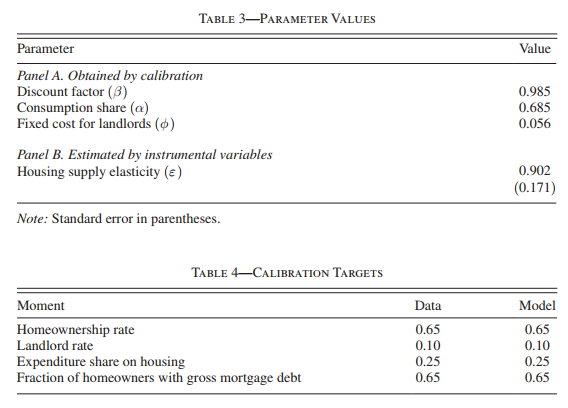
\includegraphics[width=\textwidth]{HKS-Figs/1.png}
	 \footnotesize{
	\caption*{Data sources: Saez \& Zucman (2016), Smith, Zidar \& Zwick (2019).}
	  }
\end{figure}
\end{frame}


\begin{frame}
  \frametitle{Overview}
\begin{wideitemize}
	\item examine a quantitative macro model with sharp implications for the distribution of wealth: can it match the data?
\begin{itemize}
\item its average shape
\item its evolution over time
\end{itemize}
	%\item in particular, study the role of a number of wealth-inequality determinants: tax rates, preferences, labor income, and portfolio returns---all varying across households and over time
	\item in particular, study the role of a number of wealth inequality determinants: tax rates, labor income, and portfolio returns---all varying across households and over time
	\item we discipline the model by tying all parameters to micro data
	\begin{itemize}
	\item does the benchmark framework do an adequate job?
	\end{itemize}
\end{wideitemize}
\end{frame}

%\begin{frame}
%\frametitle{Trends in wealth inequality: recent literature}
%
%\begin{itemize}
%\item {\em data:\/}
%Saez and Zucman 2015, Kopczuk 2015, Bricker, Henriques, Krimmel, and Sabelhaus 2016.
%\item
%{\em models of Pareto tails:\/}
%Piketty and Zucman 2015, Benhabib, Bisin, and Luo 2015, Nirei and Aoki 2015.
%\item {\em models of transitions:\/}
%Kaymak and Poschke 2016, Gabaix, Lasry, Lions, and Moll 2016, Aoki and Nirei 2016.
%\end{itemize}
%
%\end{frame}

\subsection{Model}
\begin{frame}
  \frametitle{Quantitative model}
	\begin{wideitemize}
		\item
		Extended Aiyagari 1994 framework:
\begin{itemize}
	\item exogenous labor supply with idiosyncratic risk: persistent and transitory component, plus Pareto tail
	\item heterogeneous returns: increasing in wealth, i.i.d.\ idiosyncratic component
	\item progressive taxation
	\item lumpsum transfer
	\item stochastic discount factor
\end{itemize}
\item time-varying: tax system, labor income process, and aggregate asset return premia
\item finding: saving rates (key consumer choice) very robust and unresponsive to all drivers
\end{wideitemize}
\end{frame}

\begin{frame}
\frametitle{Consumer problem}

\small{

\begin{align*}
	V_t(x_t,p_t,\beta_t) = & \; \max_{a_{t+1} \geq \underline{a}} \left\{u(x_t-a_{t+1}) +
	\beta_t \mathbb{E} \left[ V_{t+1}(x_{t+1},p_{t+1},\beta_{t+1}) | p_t,\beta_t \right] \right\} \\
	\text{subject to } x_{t+1} = & \; a_{t+1} + y_{t+1} - \tau_{t+1}(y_{t+1}) + (1-\tilde\tau_{t+1}) \tilde{y}_{t+1} +  T_{t+1} \\
	  y_{t+1} = & \; \left(\underline{r}_{t+1} + r^{X}_{t+1}(a_{t+1}) \right) a_{t+1} + w_{t+1} l_{t+1}(p_{t+1},\nu_{t+1}) \\
	  \tilde{y}_{t+1} = & \; \sigma^X(a_{t+1}) \eta_{t+1} a_{t+1}
\end{align*}

\begin{itemize}
\item cash-on-hand $x_t$
\item persistent component of labor income process $p_t$ and discount factor $\beta_t$ follow Markov processes
\item transitory shocks to labor income $\nu_t$ and capital income $\eta_t$
\item progressive tax on ordinary income $\tau_t(\cdot)$; flat on cap. gains $\tilde\tau_t$
\item Lumpsum transfer $T_t$
\end{itemize}

}

\end{frame}



\begin{frame}
\frametitle{Equilibrium: capital market clearing}


\begin{wideitemize}
\item need to find two equil. objects $(K_t, \underline{r}_{t})$ for capital market clearing:

\begin{enumerate}

\item aggregate capital (as usual)
$$K_t = \int a_t d \Gamma(a_t)$$

\item aggregate capital income (redundant if $r^X_{t}(\cdot)=0$)
\begin{align*}
(MPK(K_t) - \delta) K_t &=   \int \left( \underline{r}_{t} + r^X_{t}(a_{t}) \right) a_t d \Gamma(a_t)
\end{align*}
\end{enumerate}

\item for initial $(K^{\ast}_t, \underline{r}^{\ast}_{t})$ and new steady state $(K^{\ast\ast}_t, \underline{r}^{\ast\ast}_{t})$, as well as over transition $(K_t, \underline{r}_{t})_{t=t_0}^{t_1}$

\end{wideitemize}






\end{frame}


%\begin{frame} \frametitle{Multiplicative shocks and Pareto tails}
%
%\begin{itemize}
%\item linear savings rules as wealth grows large (Bewley 1977;
%Carroll 2012; Benhabib et al.\ 2015):
%$\lim_{x \rightarrow \infty} s(x,\beta) = \bar{s}_{\beta} x$.
%\item
%asset accumulation for large $x$:
%\begin{eqnarray*}
%a_{t+1} & = & s(x_t,\beta) \\
%& = & s(a_t + y_t - T(y_t),\beta) \\
%& \approx & \bar{s}_{\beta} a_t (1 + (1-\tau_{\max}) r) +
%\bar{s}_{\beta} (1-\tau_{\max}) e_t \\
%& \equiv & \hat{s} a_t + z_t,
%\end{eqnarray*}
%where $e_t$ is earnings.
%\item $\beta$ and/or $r$ random $\rightarrow$ $\hat{s}$ is random.
%\item with reflecting barrier (borrowing constraint) and/or
%random earnings, the invariant distribution for wealth has a Pareto tail with coefficient $\zeta$ solving: $\mathbb{E}[\hat{s}^\zeta] = 1$.
%\end{itemize}
%
%\end{frame}

%\begin{frame}
% \frametitle{Stochastic-$\beta$ yields stochastic, linear savings decisions}
%\begin{figure}[htbp]
%	\centering
%		 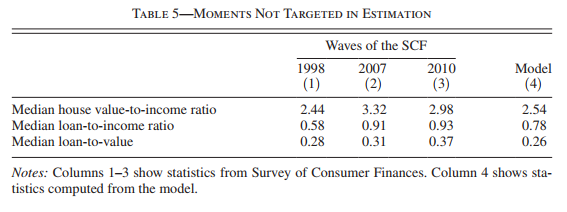
\includegraphics[width=0.95\textwidth]{HKS-Figs/2.png}
%\end{figure}
%\end{frame}
%
%\begin{frame}
% \frametitle{Gives rise to a Pareto tail in the wealth distribution}
%\begin{figure}[htbp]
%	\centering
%		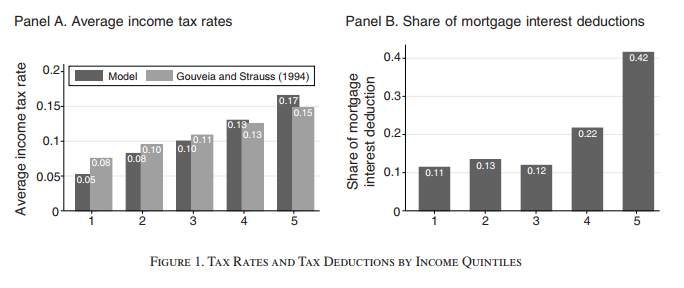
\includegraphics[width=0.95\textwidth]{HKS-Figs/3.png}
%\end{figure}
%\end{frame}

\subsection{Calibration Strategy}
\begin{frame}
  \frametitle{Calibration strategy summary}
\begin{enumerate}
\item calibrate earnings process, tax rates, return process, social safety net to observables
\pause 

\item choose randomness in discount factor $\beta$ residually so as to replicate the wealth distribution in the initial steady state (1967)
%\begin{itemize}
%\item but version without randomness in $\beta$ does almost as well
%\end{itemize}

\pause 
\item then feed in exogenous changes in tax rates, earnings inequality, etc. between 1967 and 2015 to understand the role of these different factors 

%focus on tail coefficient alone can be quite misleading: 
%\begin{itemize}
%	\item even if say the richest 10\% can be described exactly by a Pareto distribution with coefficient $\alpha > 1$, the coefficient only tells us $\forall ~ x \leq 10$: $ \frac{\text{wealth hold by top x }\%}{\text{wealth hold by top 10 }\%} = (\frac{x}{10})^\frac{\alpha-1}{\alpha}$
%	
%\item so it tells us how much wealth is concentrated within, say, the 10\%, but not overall wealth inequality (e.g. the top 1\% or top 10\% wealth share or Gini coefficient)
%\end{itemize}
\end{enumerate}
\end{frame}

\begin{frame}
\frametitle{Return heterogeneity}
\begin{wideitemize}
\item overall return given asset holdings $a_t$ equals
\begin{align}
\underline{r}_{t} + r^X_{t}(a_{t}) +  \sigma^X(a_{t}) \eta_{t} \nonumber
\end{align}
\item $\underline{r}_{t}$ is endogenous
\item $r^X_{t}(\cdot)$ and $\sigma^X(\cdot)$ are exogenous excess return schedules (mean and st.dev.), taken from the data
\item $\eta_{t}$ is an i.i.d. standard normal shock
\item reduced form portfolio choice
\end{wideitemize}
\end{frame}

\begin{frame}
  \frametitle{Calibration: return process}

  \begin{align} \nonumber
  r^X_t(a_t) = \; & \sum_{c \in C} w_c(a_t) \left(\bar{r}_{c,t} + \tilde{r}_c^X(a_t) \right) \\ \nonumber
  \left( \sigma^X(a_t) \right)^2 = \; & \sum_{c \in C} \left( w_c(a_t) \tilde\sigma^X_c(a_t) \right)^2
  \end{align}
\begin{itemize}
\item asset classes $C$: risk-free, public equity, private equity, housing
\item $\bar{r}_{c,t} $: aggregate return on asset class $c$ (U.S. data), \textcolor{blue}{time-varying}
\item fixed over time, based on Swedish administrative data from Bach, Calvet, Sodini (2016):
\begin{itemize}
\item  $w_c(\cdot)$: portfolio weights
\item $\tilde{r}_c^X(\cdot)$: within asset class return heterogeneity
\item $\tilde\sigma^X_c(\cdot)$: asset $c$ idiosyncratic return standard deviation
\end{itemize}
\end{itemize}

\end{frame}


%\begin{frame}
%\frametitle{Public and private equity}
%\textbf{Public Equity}
%\begin{itemize}
%\item U.S. stock market return
%\end{itemize}
%\textbf{Private Equity}
%\begin{itemize}
%\item Kartashova (AER, 2014) documents private equity premium over stock market
%\item aggregate time series for U.S. starting in 1960
%\end{itemize}
%\end{frame}


%\begin{frame}
%\frametitle{Housing details}
%\begin{itemize}
%\item financial return on housing as sum of capital gains term and rental income
%\item we set capital gains term to zero in steady states (in long run 0-0.5\% real price growth)
%\item over transition, use growth in aggregate house price index (Case-Shiller)
%\item rental income set to 5.33\% (average for U.S. from Jorda, Knoll, Kuvshinov, Schularick, Tayler "Rate of Return on Everything")
%\end{itemize}
%\end{frame}




\begin{frame}

\frametitle{Excess return schedule details}

\begin{itemize}
\item
Aggregate Excess Returns in 1967 steady state:
\begin{itemize}
\item public equity 0.067 (U.S., Kartashova 2014)
\item private equity 0.129 (U.S., Kartashova 2014)
\item housing  0.037 (incl. imputed rent; Jorda, et al, 2017)
\end{itemize}
\vfill
\item and cross-sectional data from Bach, Calvet, Sodini (2019) implies
\end{itemize}

% Table generated by Excel2LaTeX from sheet 'r_ex_sd'
\begin{table}[htbp]
  \centering

\resizebox{1.1\textwidth}{!}{

    \begin{tabular}{lrrrrrrrrrrrrr}
    \toprule
          & \multicolumn{1}{l}{P0-P40} & \multicolumn{1}{l}{P40-P50} & \multicolumn{1}{l}{P50-P60} & \multicolumn{1}{l}{P60-P70} & \multicolumn{1}{l}{P70-P80} & \multicolumn{1}{l}{P80-P90} & \multicolumn{1}{l}{P90-P95} & \multicolumn{1}{l}{P95-P97.5} & \multicolumn{1}{l}{P97.5-P99} & \multicolumn{1}{l}{P99-P99.5} & \multicolumn{1}{l}{P99.5-P99.9} & \multicolumn{1}{l}{P99.9-P99.99} & \multicolumn{1}{l}{Top 0.01\%} \\
    \midrule
    \multicolumn{5}{l}{fixed portfolio weights} &       &       &       &       &       &       &       &       &  \\
\cmidrule{1-5}    risk-free  & 0.722 & 0.412 & 0.248 & 0.182 & 0.156 & 0.134 & 0.115 & 0.102 & 0.090 & 0.079 & 0.071 & 0.051 & 0.029 \\
    housing & 0.162 & 0.394 & 0.580 & 0.662 & 0.678 & 0.674 & 0.658 & 0.626 & 0.572 & 0.482 & 0.363 & 0.253 & 0.155 \\
    public equity & 0.113 & 0.189 & 0.165 & 0.147 & 0.153 & 0.170 & 0.189 & 0.207 & 0.219 & 0.232 & 0.230 & 0.185 & 0.179 \\
    private equity & 0.002 & 0.005 & 0.007 & 0.009 & 0.013 & 0.021 & 0.038 & 0.065 & 0.118 & 0.207 & 0.336 & 0.511 & 0.637 \\
    \midrule
%    \multicolumn{5}{l}{difference from aggregate return on asset class } &       &       &       &       &       &       &       &       &  \\
%\cmidrule{1-5}    risk-free  & 0.000 & 0.000 & 0.000 & 0.000 & 0.000 & 0.000 & 0.000 & 0.000 & 0.000 & 0.000 & 0.000 & 0.000 & 0.000 \\
%    housing & 0.000 & 0.000 & 0.002 & 0.004 & 0.005 & 0.007 & 0.009 & 0.010 & 0.010 & 0.011 & 0.010 & 0.010 & 0.011 \\
%    public equity & 0.000 & 0.000 & 0.001 & 0.002 & 0.003 & 0.005 & 0.008 & 0.012 & 0.014 & 0.015 & 0.016 & 0.016 & 0.016 \\
%    private equity & 0.000 & 0.000 & -0.019 & -0.030 & -0.054 & -0.055 & -0.049 & -0.066 & -0.064 & -0.063 & -0.063 & -0.059 & -0.060 \\
%    \midrule
%    \multicolumn{5}{l}{standard deviation of return on asset class} &       &       &       &       &       &       &       &       &  \\
%\cmidrule{1-5}    risk-free  & 0.000 & 0.000 & 0.000 & 0.000 & 0.000 & 0.000 & 0.000 & 0.000 & 0.000 & 0.000 & 0.000 & 0.000 & 0.000 \\
%    housing & 0.140 & 0.140 & 0.140 & 0.140 & 0.140 & 0.140 & 0.140 & 0.140 & 0.140 & 0.140 & 0.140 & 0.140 & 0.140 \\
%    public equity & 0.035 & 0.035 & 0.031 & 0.031 & 0.031 & 0.031 & 0.032 & 0.033 & 0.035 & 0.038 & 0.042 & 0.046 & 0.053 \\
%    private equity & 0.664 & 0.664 & 0.621 & 0.595 & 0.544 & 0.525 & 0.518 & 0.480 & 0.474 & 0.470 & 0.474 & 0.492 & 0.443 \\
%    private equity (re-scaled) & 0.345 & 0.345 & 0.323 & 0.309 & 0.283 & 0.273 & 0.269 & 0.249 & 0.246 & 0.245 & 0.246 & 0.256 & 0.230 \\
%    \midrule
%    \multicolumn{5}{l}{excess return schedule in 1967} &       &       &       &       &       &       &       &       &  \\
%\cmidrule{1-5}    mean excess return & 0.000 & 0.011 & 0.017 & 0.020 & 0.022 & 0.026 & 0.031 & 0.035 & 0.041 & 0.050 & 0.062 & 0.079 & 0.091 \\
%    standard deviation & 0.023 & 0.056 & 0.081 & 0.093 & 0.095 & 0.095 & 0.094 & 0.093 & 0.098 & 0.119 & 0.167 & 0.254 & 0.283 \\
%    st. dev. (priv.equ. re-scaled) & 0.023 & 0.056 & 0.081 & 0.093 & 0.095 & 0.095 & 0.093 & 0.089 & 0.086 & 0.085 & 0.098 & 0.136 & 0.149 \\
    \bottomrule
    \end{tabular}%

}

\end{table}%

\end{frame}



\begin{frame}
\frametitle{Schedule of excess returns}

\begin{figure}
	\centering
		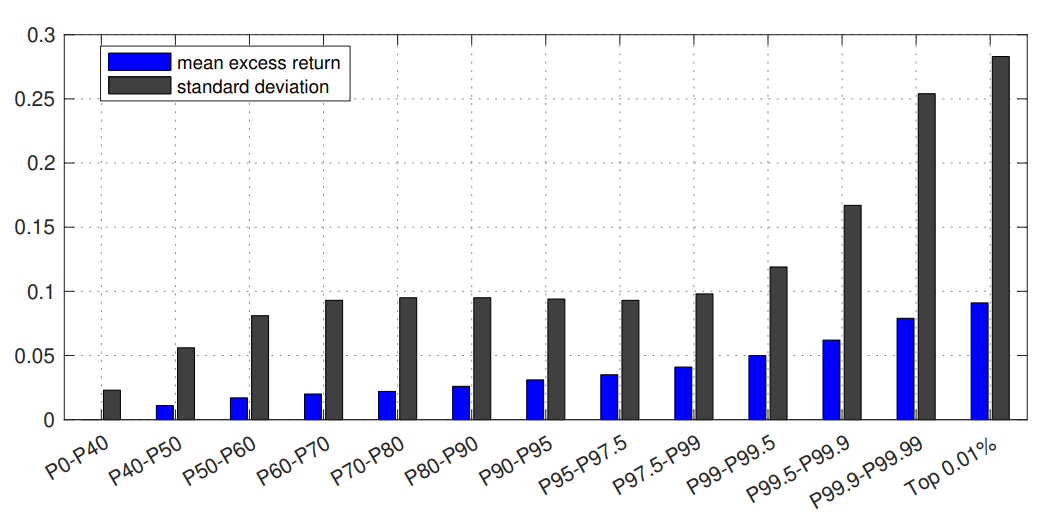
\includegraphics[width=\textwidth]{HKS-Figs/4.png}
	 \footnotesize{
	\caption*{Data sources: Bach, Calvet, Sodini (2019); Kartashova (2014); Jorda, Knoll, Kuvshinov, Schularick, Taylor (2019); Case-Shiller.}
	  }
\end{figure}

\end{frame}




\subsection{Results}
\begin{frame}
  \frametitle{Results, I: steady state (1967)}
		
\begin{table}[htbp]
  \centering
\resizebox{\textwidth}{!}{
     \begin{tabular}{lrrrr}
    \toprule
          & Top 10\% & Top 1\% & Top 0.1\% & Top 0.01\% \\
    \midrule
    Data & 70.8\% & 27.8\% & 9.4\% & 3.1\% \\
    Single-$\beta$ Model & 66.6\% & 23.7\% & 11.2\% & 7.2\% \\
    Benchmark Model & 73.8\% & 27.4\% & 8.4\% & 3.2\% \\
    \midrule
          & Bottom 50\% & Fraction $a<0$ &       &  \\
    \midrule
    Data & 4.0\% & 8.0\% &       &  \\
    Single-$\beta$ Model & 3.5\% & 7.3\% &       &  \\
    Benchmark Model & 3.0\% & 6.6\% &       &  \\
    \bottomrule
    \end{tabular}}%
\end{table}%

\begin{itemize}
\item model matches wealth distribution well on its entire domain
\begin{itemize}
\item return heterogeneity is key ingredient
\item wealth concentration is mitigated by progressive taxation and labor income risk
\end{itemize}
\end{itemize}
\end{frame}



\begin{frame}
\frametitle{Next step: transition}
The authors feed in four different factors that have changed during the past 50 years
\begin{wideitemize}
	\item Decrease in tax progressivity 
	\item Increase in labor income risk
	\item Increase in income going to the top 
	\item Changing return premia to different asset classes
\end{wideitemize}
\vfill \pause
Note: in two weeks, we will learn more about the solution method for solving for the transition from one steady state to another
\end{frame}


\begin{frame}
  \frametitle{Observed change 1: decrease in tax progressivity}
	\begin{itemize}
		\item federal effective tax rates (Piketty \& Saez 2007): income, payroll, corporate and estate taxes
	\end{itemize}
	\begin{figure}[htbp]
	\centering
		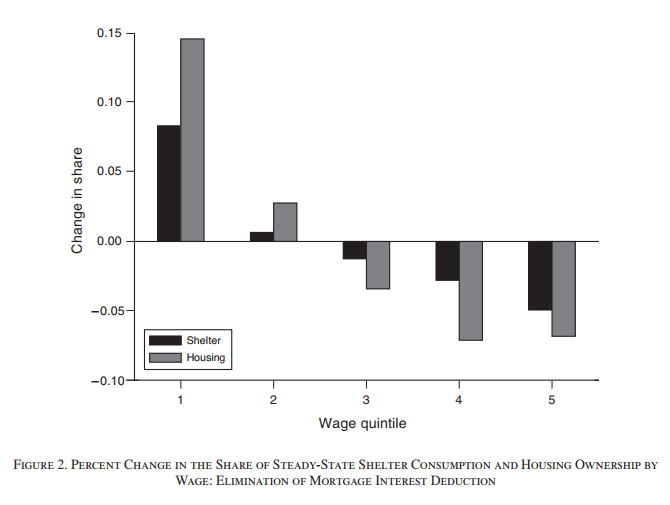
\includegraphics[width=0.8\textwidth]{HKS-Figs/5.png}
		\end{figure}
\end{frame}

\begin{frame}
\frametitle{Observed change 2: increase in labor income risk}
		\begin{itemize}
			\item estimates for variance of persistent and temporary components 1967-2000 (Heathcote, Storesletten \& Violante 2010)
		\end{itemize}
	\begin{figure}[htbp]
	\centering
		 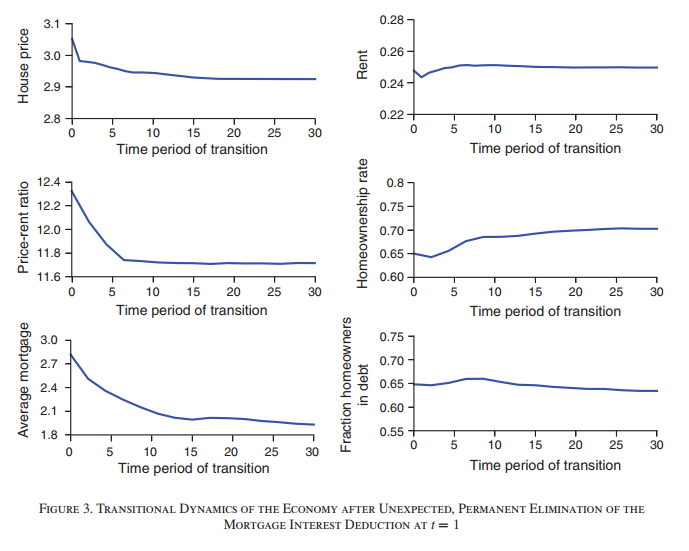
\includegraphics[width=0.8\textwidth]{HKS-Figs/6.png}
		\end{figure}
\end{frame}

\begin{frame}
\frametitle{Observed change 3: increase in top labor income shares}
		\begin{itemize}
			\item adjust standard AR(1) in idiosyncratic productivity by imposing a Pareto tail for the top 10\% earners: calibrated tail coefficient decreases from 2.8 to 1.9 (updated Piketty \& Saez 2003 series)
		\end{itemize}
	\begin{figure}[htbp]
	\centering
		 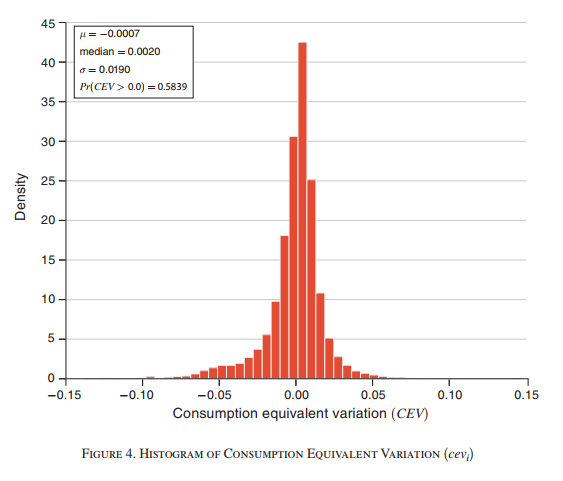
\includegraphics[width=0.8\textwidth]{HKS-Figs/7.png}
		\end{figure}
\end{frame}


\begin{frame}
\frametitle{Observed change 4: return premia}
		\begin{wideitemize}
			\item feed in (smoothed) time series of aggregate U.S. asset premia (Kartashova 2014, Case-Shiller index)
		\end{wideitemize}
		\visible<2->{
	\begin{figure}[htbp]
	\centering
		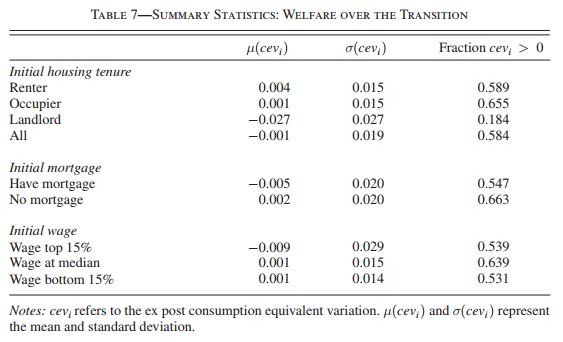
\includegraphics[width=1.0\textwidth]{HKS-Figs/8.png}
		\end{figure} }
\end{frame}


\begin{frame}
\frametitle{Observed change 4: return premia}
		\begin{wideitemize}
			\item feed in (smoothed) time series of aggregate U.S. asset premia (Kartashova 2014, Case-Shiller index)
		\end{wideitemize}
	\begin{figure}[htbp]
	\centering
		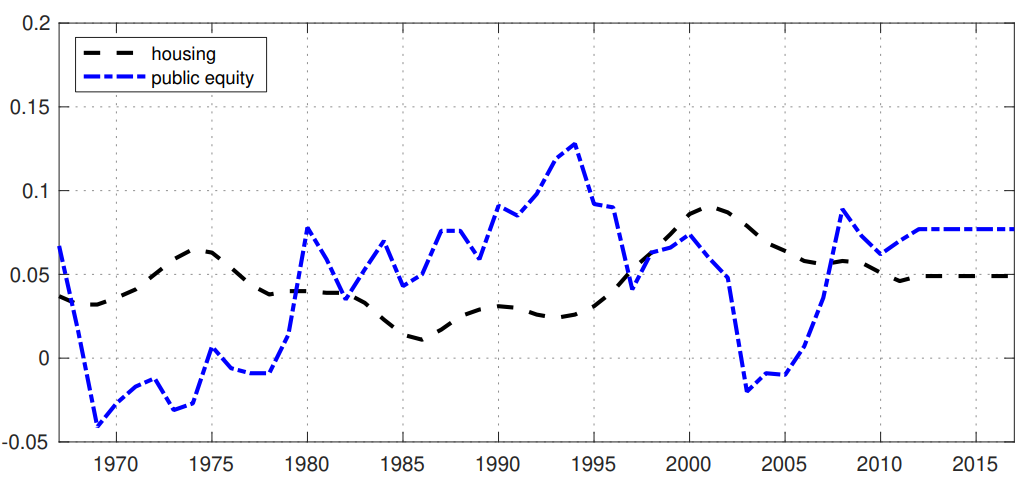
\includegraphics[width=1.0\textwidth]{HKS-Figs/9.png}
		\end{figure}
\end{frame}


\begin{frame}
\frametitle{Observed change 4: return premia}
		\begin{wideitemize}
			\item feed in (smoothed) time series of aggregate U.S. asset premia (Kartashova 2014, Case-Shiller index)
		\end{wideitemize}
	\begin{figure}[htbp]
	\centering
		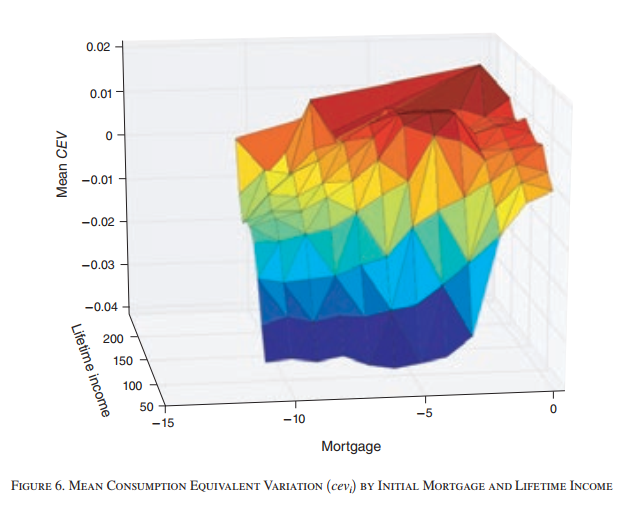
\includegraphics[width=1.0\textwidth]{HKS-Figs/10.png}
		\end{figure}
\end{frame}



\begin{frame}
  \frametitle{Results, II: historical evolution}
		\begin{figure}[htbp]
	\centering
		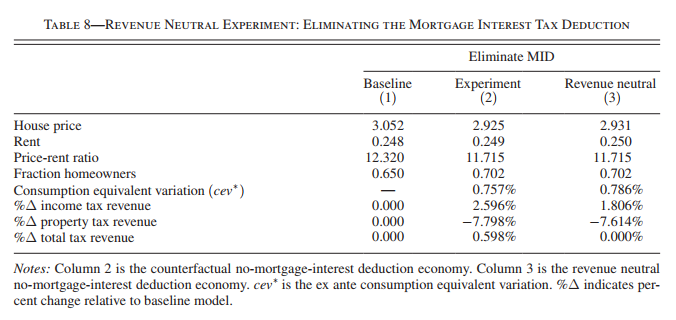
\includegraphics[width=1.0\textwidth]{HKS-Figs/11.png}
\end{figure}
\end{frame}

%%% other results


\begin{frame}
  \frametitle{Results: Capital-output ratio and bottom 50 \%}
		\begin{figure}[htbp]
	\centering
		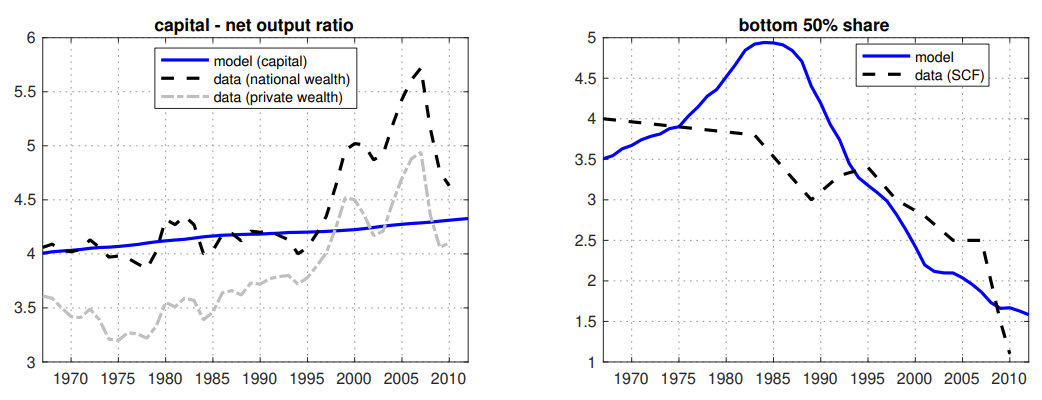
\includegraphics[width=1.0\textwidth]{HKS-Figs/12.png}
\end{figure}
\end{frame}

\begin{frame}
  \frametitle{Results: Risk-free rate}
  \begin{itemize}
  \item return premia are matched in model by construction
  \item risk-free rate is endogenous: comparable level and decline
  \end{itemize}
		\begin{figure}[htbp]
	\centering
		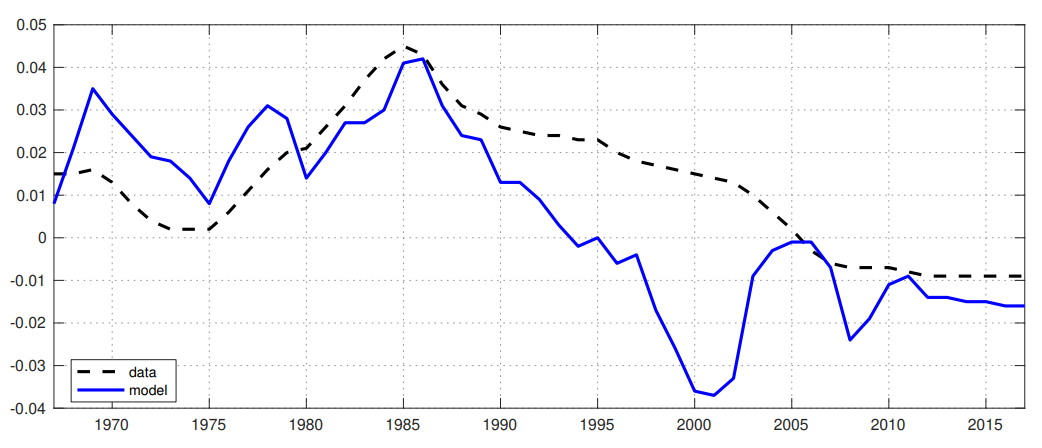
\includegraphics[width=1.0\textwidth]{HKS-Figs/13.png}
\end{figure}
\end{frame}


\begin{frame}
  \frametitle{Decomposition of transitional dynamics}
		\begin{figure}[htbp]
	\centering
		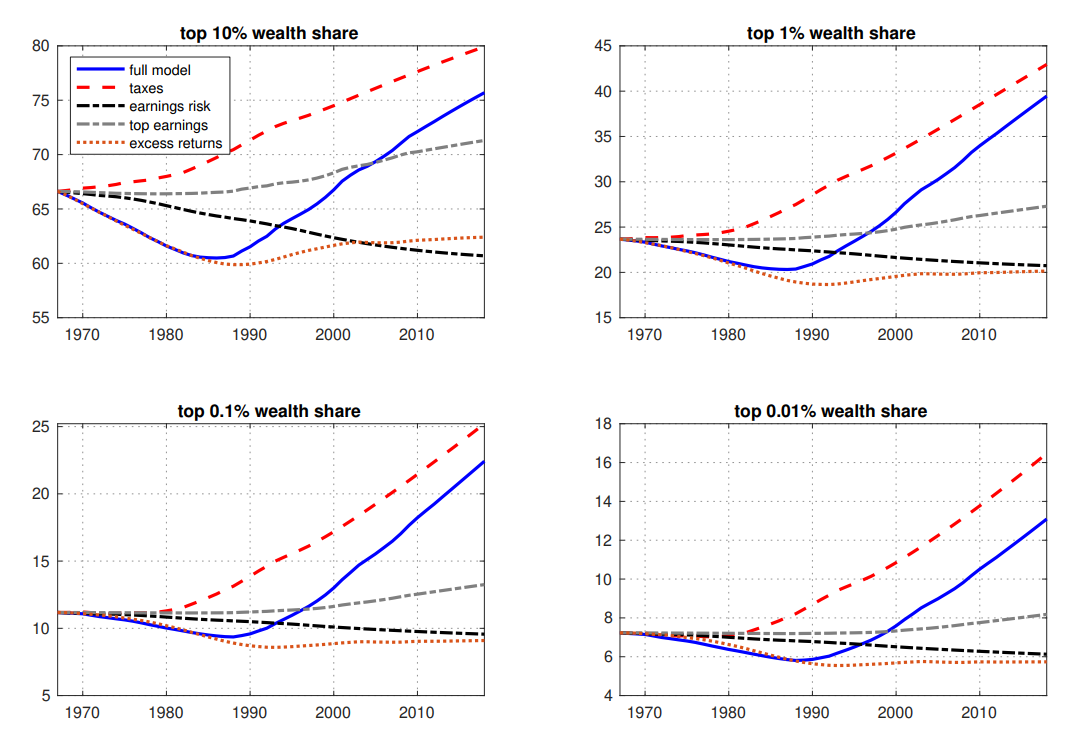
\includegraphics[width=1.0\textwidth]{HKS-Figs/14.png}
\end{figure}
\end{frame}

%%%%%%%%%%%%%%%%%%%%%%%%%%%%%%%%%%%%%%%%%%%%%%%%%%
%                            Multiple-beta Model Transition
%%%%%%%%%%%%%%%%%%%%%%%%%%%%%%%%%%%%%%%%%%%%%%%%%%
%
%\begin{frame}
%  \frametitle{Dynamics in multiple-$\beta$ model I}
%  only some level difference in richer benchmark model (paper):
%		\begin{figure}[htbp]
%	\centering
%		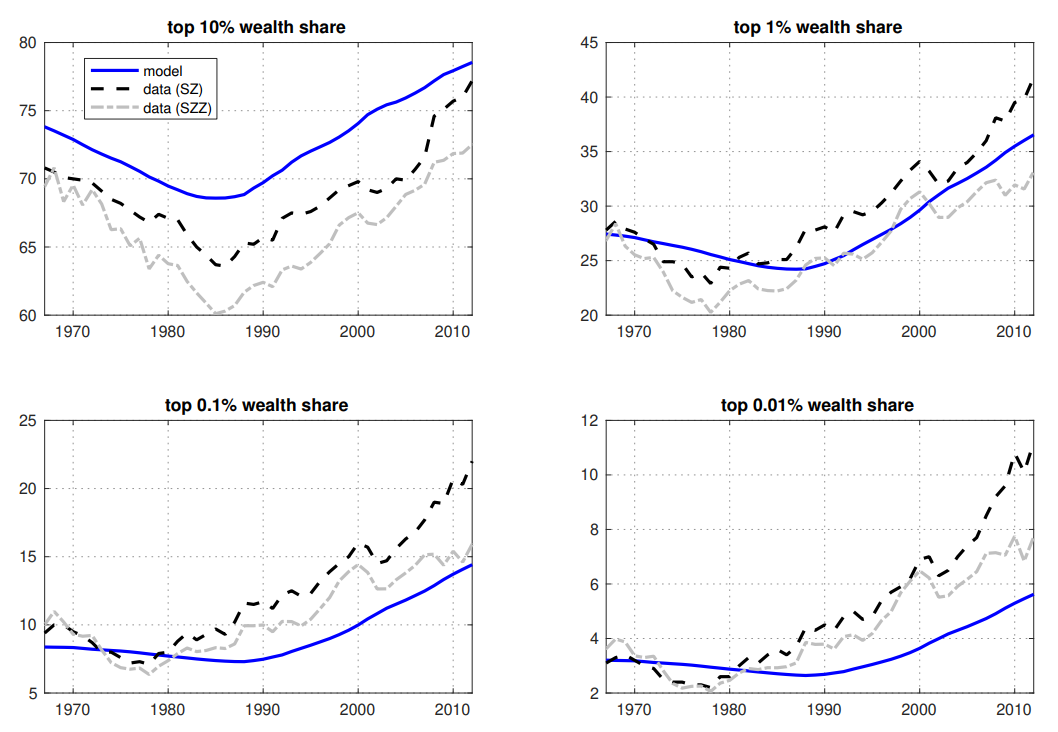
\includegraphics[width=1.0\textwidth]{HKS-Figs/15.png}
%\end{figure}
%\end{frame}
%
%\begin{frame}
%  \frametitle{Dynamics in multiple-$\beta$ model II}
%		\begin{figure}[htbp]
%	\centering
%		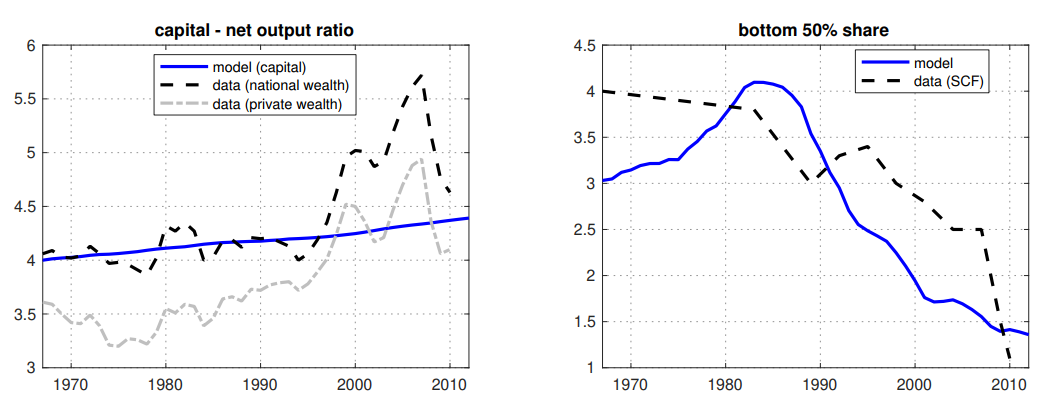
\includegraphics[width=1.0\textwidth]{HKS-Figs/16.png}
%\end{figure}
%\end{frame}
%
%
%\begin{frame}[label=summary]
%\frametitle{Summary of transitional dynamics}
%\begin{wideitemize}
%	\item model captures the salient features of the evolution of the U.S.\ wealth distribution
%	\item these results are robust
%	\begin{itemize}
%	\item perfect foresight not critical 
%	\item robust to CES production function with elasticity $>1$ and more generally falling labor share 
%\end{itemize}
%\item shortcomings:
%\begin{itemize}
%\item explosion of wealth concentration at the extreme top (0.01\%) not fully captured quantitatively
%\end{itemize}
%\end{wideitemize}
%\end{frame}

		
\begin{frame}[label=decomposemain]
\frametitle{Decomposition of transitional dynamics}
\begin{wideitemize}
	\item overall increase in wealth inequality (more than) fully explained by declining tax progressivity
	\begin{itemize}
	\item primarily due to direct effect on resource distribution and not due to changing savings behavior 
	\end{itemize}
	\item time-varying return premia account for U-shape in wealth inequality
	\item subtle role of increasing earnings dispersion
	\begin{itemize}
	\item thickening Pareto tail in labor income contributes slightly positively to wealth inequality
	\item increase in overall earnings risk decreases wealth inequality
	\end{itemize}
\end{wideitemize}
\end{frame}


\begin{frame}
  \frametitle{Capital in the 21st century?}
\begin{figure}[htbp]
	\centering
		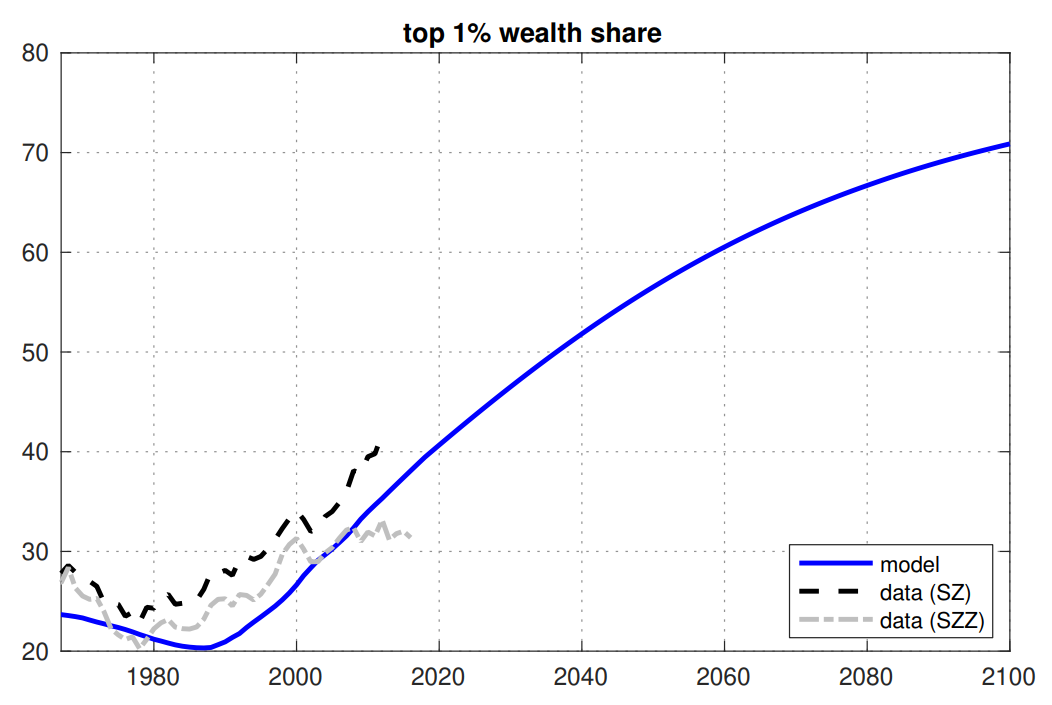
\includegraphics[width=1.0\textwidth]{HKS-Figs/17.png}
\end{figure}
\end{frame}

\begin{frame}
\frametitle{
Conclusion}

\begin{wideitemize}
\item<1-> the model does a good job at accounting for the level of wealth inequality
\begin{itemize}
\item (realistic) return heterogeneity is key
\end{itemize}
\item<2-> the model does a good job at explaining its evolution over time
\begin{itemize}
\item declining tax progressivity most powerful force for generating increases in wealth inequality
\item
asset-price movements account well for medium-run dynamics
\end{itemize}
\item<3-> cautious prediction: unless stronger tax progressivity restored, wealth concentration will continue to rise

\end{wideitemize}
\end{frame}



\section{Summary}
\begin{frame}{Summary and next week}
\begin{wideitemize}
	\item <+->\textbf{Today:} Discussed the predictions for wealth inequality arising from Bewley-Huggett-Aiyagari models and their various extensions
	\begin{enumerate}
		\item Difficult to match the fact that wealth more unequal than earnings
		\item Heterogeneity in returns seems very important
		\item Then analyzed the rise in wealth inequality in the US
	\end{enumerate}
	\item <+->\textbf{Next week: } Learn to extend the workhorse model to include equilibrium in housing markets
%	\item <+->\textbf{Homework:} Begin work on the first assignment 
\end{wideitemize}

\end{frame}


\end{document} 